\documentclass{beamer}
\usetheme{Madrid}
\usepackage{bm}
\usepackage{pgfplots}
\pgfplotsset{compat=1.15}
\usepackage{mathrsfs}
\usetikzlibrary{arrows}
\usepackage[utf8]{inputenc}
\usepackage{xcolor}
\usepackage{nicematrix}
\usepackage{tikz}
\usepackage{comment}
\usepackage{hyperref}
\usepackage{fancyvrb}
\usepackage{mathtools}
\usepackage{comment}
\usepackage{array}
\usepackage{pgfcore}
\usepackage{listings}
\usepackage{color}
\definecolor{munsell}{rgb}{0.0, 0.5, 0.69}
\definecolor{dkgreen}{rgb}{0,0.6,0}
\definecolor{gray}{rgb}{0.5,0.5,0.5}
\definecolor{mauve}{rgb}{0.58,0,0.82}
\definecolor{minas}{RGB}{0.244, 0.172, 0.36}
\definecolor{PUJ}{RGB}{44, 86, 151}
\definecolor{PUJ2}{RGB}{43, 93, 156}
\definecolor{PUJ3}{RGB}{20, 52, 107}
\definecolor{cyandk}{rgb}{0.0, 0.72, 0.92}
\setbeamerfont{frametitle}{size=\LARGE ,series=\bfseries}
\setbeamercolor{frametitle}{fg=PUJ2, bg=white} %% title of the beamer
\setbeamercolor{titlelike}
{parent=structure,bg=PUJ2}
\setbeamercolor{title}{fg=white, bg=PUJ3} 
%\setbeamercolor{navigation symbols}{fg=white, bg=white}
\setbeamercolor*{palette primary}{use=structure,fg=black,bg=yellow}
\setbeamercolor*{palette secondary}{use=structure,fg=white,bg=PUJ3}
\setbeamercolor*{palette tertiary}{use=structure,fg=white,bg=PUJ3}

\setbeamercolor{block title}{bg=PUJ3,fg=white}


%% code information
\lstset{frame=tb,
  language=Python,
  aboveskip=3mm,
  belowskip=3mm,
  showstringspaces=false,
  columns=flexible,
  basicstyle={\small\ttfamily},
  numbers=none,
  classoffset=1,
  morekeywords={True,False}, keywordstyle=\color{munsell}, 
  classoffset=0, 
  keywordstyle=\color{blue},  
  commentstyle=\color{dkgreen},
  stringstyle=\color{PUJ3},
  numberstyle=\tiny\color{gray},
  breaklines=true,
  breakatwhitespace=true,
  tabsize=4,
}

%% You can change default language in the middle of document with \lstset{language=Java}.


%% PUT or Remove the logo in a slide.


%% Information topic

\institute{Javeriana}
\date{2020}

\title[Pontificia Universidad Javeriana] %optional
{Introduction to Perceptron}
\subtitle{ using python.}

\author[Iván Andrés Trujillo] 
{
Iván Andrés Trujilllo Abella}

\institute[] 
{
  Facultad de Ingenieria\\
  Pontificia Universidad Javeriana
  \and
  
\textbf{ trujilloiv@javeriana.edu.co \\
addajaveriana}
}

\date[MINTA] % (optional)

\newif\ifplacelogo % create a new conditional
\placelogotrue % set it to true
%\logo{\ifplacelogo\color{red}\rule{.5cm}{.5cm}\fi}
\logo{\ifplacelogo 
\includegraphics[height= 2.0cm]{pujshield.eps}\fi}



\begin{document}



\frame{\titlepage}


\begin{frame}[fragile]{Background classification problem}
Fisher(1936) proposes the linear Discriminant, 
the problem consist in predict a binary outcome according to a set of features, for instance find the variables that could predict the bankruptcy.

The main objective is construct a $z = \mathbf{w^{t}x}$ 
score whose indicate the probability of belonging to a class.
\end{frame}


\begin{frame}{Binary classification problem}
$y_{0},y_{1} \in Y $ and $y_{0} \cup y_{1} = Y$ and $y_{0} \cap y_{1} = \emptyset$ both class are exhaustive and are defined without ambiguity. 
A vector of weights and a vector of features for a 
\[
w^{t} \mathbf{x} = 
\begin{bmatrix}
w_{1} \\
w_{2} \\
\vdots \\
\end{bmatrix}
\begin{bmatrix}
x_{1} & x_{2} & \cdots & x_{n}
\end{bmatrix}
= \sum_{i=1}^{n}w_{i}x_{i} = z_{i}
\]

\end{frame}

\begin{frame}[fragile]{Perceptron}
Rossenblant(1958)
We can define a vector input $\mathbf{x}$ and a vector of weights $\mathbf{w}$ and a activation function $\varphi$ that take as input the inner product of both vectors defined previously $\varphi(\mathbf{w}^{t}\mathbf{x})$.

\end{frame}



\begin{frame}
\tikzset{basic/.style={draw,fill=none,
                       text badly centered,minimum width=3em}}
\tikzset{input/.style={basic,circle,minimum width=3.5em}}
\tikzset{weights/.style={basic,rectangle,minimum width=2em}}
\tikzset{functions/.style={basic,circle, minimum width=4em}}
\newcommand{\addaxes}{\draw (0em,1em) -- (0em,-1em)
                            (-1em,0em) -- (1em,0em);}
\newcommand{\relu}{\draw[line width=1.5pt] (-1em,0) -- (0,0)
                                (0,0) -- (0.75em,0.75em);}
\newcommand{\stepfunc}{\draw[line width=1.5pt] (0.65em,0.65em) -- (0,0.65em) 
                                    -- (0,-0.65em) -- (-0.65em,-0.65em);}
    \begin{tikzpicture}[scale=1.2]
    % Draw input nodes
    \foreach \h [count=\hi ] in {$x_2$,$x_1$,$x_0=1$}{%
          \node[input] (f\hi) at (0,\hi*1.25cm-1.5 cm) {\h};
        }
    % Dot dot dot ... x_n
    \node[below=0.62cm] (idots) at (f1) {\vdots};
    \node[input, below=0.62cm] (last_input) at (idots) {$x_n$};
    % Draw summation node
    \node[functions] (sum) at (4,0) {\Huge$\sum$};
    \node[below=0.69cm] at (sum) {$z = \sum_{i=0}^n w_ix_i$};
    % Draw edges from input nodes to summation node
    \foreach \h [count=\hi ] in {$w_2$,$w_1$,$w_0$}{%
          \path (f\hi) -- node[weights] (w\hi) {\h} (sum);
          \draw[->] (f\hi) -- (w\hi);
          \draw[->] (w\hi) -- (sum);
        }
    % Dot dot dot ... w_n
    \node[below=0.05cm] (wdots) at (w1) {\vdots};
    \node[weights, below=0.45cm] (last_weight) at (wdots) {$w_n$};
    % Add edges for last node and last weight etc
    \path[draw,->] (last_input) -- (last_weight);
    \path[draw,->] (last_weight) -- (sum);
    % Draw node for activation function
    \node[functions] (activation) at (7,0) {};
    % Place activation function in its node
    \begin{scope}[xshift=7cm,scale=1.25]
        \addaxes
        % flexible selection of activation function
        \stepfunc
        % \stepfunc
    \end{scope}
    % Connect sum to relu
    \draw[->] (sum) -- (activation);
    \draw[->] (activation) -- ++(1,0);
    % Labels
    \node[above=1cm]  at (f3) {inputs};
    \node[above=1cm] at (w3) {weights};
    \node[above=1cm] at (activation) {activation function  $\varphi(z)$};
    \end{tikzpicture}
\end{frame}



\begin{frame}[fragile]{Activation function}
$\varphi()$ could be defined as the sigmoid function.

\begin{equation}
\begin{align*}
p(y=1) = \varphi(z) \\
p(y=0) = 1 -\varphi(z)
\end{align*}
\end{equation}
Percepton works with a step function:

\begin{equation*}
\varphi(z) = 
    \begin{dcases}
        0 &  z < 0 \\
        1 &  z \geq 0
    \end{dcases}
\end{equation*}    
Returning  a binary outcome.
\end{frame}


\begin{frame}{What set of $w$ values we must choose}{Cost function}
The cost function could be defined in a soft or a hard way.
\begin{equation}
J(w)_{hard} = \sum_{i=1}^{n} = \max(-y_{i}\hat{y},0)
\end{equation}
$J$ only count the number of mismatches.
However this function not is differentiable.

\begin{equation}
J(w)_{soft} = \sum_{i=1}^{n} = \max(-y_{i} z_{i},0)
\end{equation}
if $y_{i}z_{i} < 0 $  then lost function $>0$

if $y_{i}z_{i}>0 $  the lost function $=0$.

\end{frame}




\begin{frame}[fragile]{Insights}

The update of weights is according to the data bias or mistakes, however when the model match to the class then
\begin{equation}
\Delta w_{i} = (y_{i} -\hat{y_{i}}) = 0
\end{equation}
where $y_{i}$ is the real observed data, and $\hat{y_{i}}$ is the predicted class.

when the $y_{i} = -1$ and $\hat{y} = 1$ then $\Delta w = -2$, in otherwise $y_{i}=1$ and $\hat{y_{i}}=-1$ then $\Delta w = 2$.
in summary:

\begin{equation*}
\Delta w_{i} = 
    \begin{dcases}
        0 &  y_{i} = \hat{y_{i}} \\
       -2 &  y_{i}<\hat{y_{i}}  \\
         2 &  y_{i}>\hat{y_{i}}
    \end{dcases}
\end{equation*}    
\end{frame}


\begin{frame}{insights}
Then when there are mistakes 
\begin{equation}
\varphi(w^{t}_{i+1} \mathbf{x_{i}}) =\varphi((w_{i} + \Delta w_{i})^{t} \mathbf{ x_{i}}) = y_{i} 
\end{equation}
This mean that  weights for the vector of features of the sample $i$ are update to predict the correct class.
 
\begin{equation}
w_{i+1} = w_{i} + \eta \Delta w_{i} \mathbf{x_{i}}
\end{equation}

\end{frame}


\begin{frame}[fragile]{Perceptron algorithm}
\begin{verbatim}
initialize w:
for each x in sample :
	estimate y(x)
	w = w + update(w)
\end{verbatim}
\end{frame}

\begin{frame}{LAB}{Perceptron implementation from scratch}
\begin{Large}
\textbf{
\href{https://colab.research.google.com/drive/13yt7cav6wZbMrmwGxjxzPKwgo5636YUj?usp=sharing}{Perceptron from scratch(click here)}}
\end{Large}
\end{frame}



\begin{frame}{sklearn}
It is open source library, integrated with scipy and numpy. It is one of the most popular machine learning library on Github. 

\begin{itemize}
\item Classification  (Neural networks
 Support Vector Machine)
\item Decision trees
\item Cluster
\item Regression
\end{itemize} 

\end{frame}

\begin{frame}[fragile]{sklearn}
\begin{lstlisting}
from skelearn.linear_model import Perceptron
model = Perceptron(penalty=None , max_iter=1000, eta0=0.4, random_state=1)
model.fit(X,y)
model.score(X,y) # Print the number of matches
from sklearn.metrics import confusion_matrix
confusion_matrix(y, model.predict(X))
print(model.coef_)
\end{lstlisting}
\end{frame}


\begin{comment}


\begin{frame}{descent gradient}
An algorithm to optimization.
We can think in a greedy algorithm, searching points, for instance to fit a line to a data points, 
$e(\beta_{0}^{v}, \beta_{1}^{f})$
then we have an associeted error fo $\beta_{0}$ $e_{\beta_{0}^{v}} =\sum_{i=1}^{n} (y_{i} - \beta_{0}^{v}+ \beta_{1}^{f}x_{i} )^{2}$. 
\end{frame}


\begin{frame}[fragile]{Binary system}
A bit is a variable that could take two possible variables $0$ and $1$ therefore $n$ bits have $2^{n}$ possibles combinations.

Remember that $10$ is $2$, the number $100$  is $4$, the number $1010$ is $10$, the convertion of decimal system to binary system.
\end{frame}



\begin{frame}{ideas over information}
a certain event don yield information, a rare event yield more information, if two events are measured apart, the information yielded is the sum of two information separately.

\end{frame}



\begin{frame}[fragile]{Entropy}
a mesaure of not order. the uncertainty, for instance suppose that you flip a coin and maximun entropy is reached when the success have $p=\frac{1}{2}$ due we do not have additional information about what side lands.

\end{frame}


\begin{frame}[fragile]{Insights about entropy}
The event with small probability of occurrence give more information than those with a major probability.


\begin{itemize}
\item jensen inequality
\item Gibbs inequality
\end{itemize}

\end{frame}



\begin{frame}
\begin{equation}
\begin{align*}
I(x) &= log \frac{1}{p(x)}
     &= - log p(x)
\end{align*}
\end{equation}
the avarage surprisal:
\begin{equation}
\sum p(x)I(x)
\end{equation}
we can rewrite as:
\begin{equation}
H(x) = - \sum p(x) log p(x)
\end{equation}
suppose that we have a variable $x \sim N(\mu, \sigma)$
do not have more entropy than a variable $y \sim U(a,b)$ given that each 'character' have the same probability of occur.
\end{frame}


\begin{frame}{Entropy in Bernouilli trial}

\begin{equation}
H(x) - \sum_{k=1}^{2} \frac{1}{2} log_{2} \frac{1}{2} = 1
\end{equation}
Note that $p_{1}=1/2$ and $p_{2} = 1/2$.

\end{frame}



\begin{frame}{Conditional entropy}
\begin{equation}
H(X \mid Y ) = \sum_{i,j}p(x_{i},y_{j})log \frac{p(x_{i},y_{j})}{p(y_{j})}
\end{equation}
\end{frame}



\begin{frame}[fragile]{Gini coefficient}
A measure of dispersion, 
A measure of inequality based upon the lorentz curve, whose is a basic but smart idea, axis represent the cumulative proportion of the variable, in the cumulative entities( persons, regions, and so on).

\end{frame}



\begin{frame}{lorentz curve}
\definecolor{qqqqcc}{rgb}{0,0,0.8}
\definecolor{qqwuqq}{rgb}{0,0.39215686274509803,0}
\begin{tikzpicture}[line cap=round,line join=round,>=triangle 45, scale=0.7]
\begin{axis}[
x=1cm,y=1cm,
axis lines=middle,
xmin=-0.1,
xmax=13.5,
ymin=0,
ymax=11,
xtick={0},
ytick={0},]
\clip(-0.8694140372315902,-4.314718926642073) rectangle (26.594349777827446,19.594337869801166);
\draw [line width=2pt,color=qqwuqq] (0,0)-- (13.16,11.1);
\draw [rotate around={-56.694479071423174:(-215.18175234556708,339.0826607244106)},line width=1.6pt,pattern color=qqqqcc] (-215.18175234556708,339.0826607244106) ellipse (402.68437368747675cm and 84.90521670471614cm);
\draw [line width=1.4pt,dotted] (13.080575941403652,11.028023396032836)-- (13,0);
\end{axis}
\end{tikzpicture}
\end{frame}


\begin{frame}[fragile]{Gini Coefficient}
Gini was defined as the area between  the line of perfect inequality and the lorentz curve  over the total area over the perfect inequality.
\begin{equation}
G = \frac{\int x dx - \int L(x)dx}{\int x dx}
\end{equation}
Note that the perfect equality line it is $y=x$ and we can said that $\int_{0}^{1} x dx =\frac{1}{2}$ due the are of triangle it is the half of the square with one dimension. Therefore:
\begin{equation}
G =  1 - 2 \int_{0}^{1} L(x) dx
\end{equation} 

the term equidistribution line.
\end{frame}




\begin{frame}{compute Gini index}
if we have $n$ observations then $Y = \sum_{j=1}^{n} y_{i}$, and assuming that $y_{1} \leq y_{2} ... \leq y_{n}$, the $l_{i} = \frac{\sum_{j=1}^{i} y_{j}}{Y}$  that is the cumulative income, equally the portion $x_{i} = \frac{i}{n}$.

then we search alternative calculate the gini index.
using one approximation we can define:
\begin{equation}
G = 1 - \sum (l_{i} + l_{i+1}) (x_{i+1} -x_{i})
\end{equation}
Notice that the trapecium are could be approximate as $((x_{i+1} - x_{i})l_{i} + (x_{i+1}-x_{i})l_{i+1})\frac{1}{2}$.
\end{frame}





\begin{frame}[fragile]{Python implementation I}
\begin{lstlisting}
def gini(array):
  # We must exclude 0 incomes?
  array.append(0)
  array = sorted(array)
  persons = len(array)-1
  acumulative_person = [x/persons for x in range(0,persons+1)]
  acumulative=[]
  count = 0
  for x in array:
    count = count + x
    acumulative.append(count)
  acumulative = [x/sum(array) for x in acumulative]
  
\end{lstlisting}
\end{frame}


\begin{frame}[fragile]{Python implementation II}
\begin{lstlisting}
# Gini 
  areas = []
  for i in range(0,len(array)-1):
      areas.append((acumulative[i+1]+acumulative[i]) *
	(acumulative_person[i+1]-acumulative_person[i]))
  gini = 1-sum(areas)
  return acumulative , acumulative_person, gini
x,y, gini = gini(incomes)
plt.plot(y,x)
plt.plot(x,x)

\end{lstlisting}
\end{frame}




\begin{frame}[fragile]{example}
\begin{lstlisting}
from math import log2
log2(1/2)
\end{lstlisting}
\end{frame}

\begin{frame}[fragile]{Theil index}
\begin{lstlisting}
from math import log
def theil(array):
  n = len(array)
  ymean = sum(array)/n
  data = [(x/ymean, log(x/ymean)) for x in array]
  Theil = sum([x[0]*x[1] for x in data])/n
  return Theil
\end{lstlisting}
\end{frame}




\begin{frame}[fragile]{Lost function}


\end{frame}



\begin{frame}{Research}
binary entropy function, log loss function.


\end{frame}


\begin{frame}
\begin{columns}
\column{0.5\textwidth}
\definecolor{qqqqcc}{rgb}{0,0,0.8}
\begin{tikzpicture}[line cap=round,line join=round, scale=0.8]
\clip(3.0110668914628027,-0.46146921060576085) rectangle (11.868629834326168,5.231022157124454);
\draw [shift={(3,1)},line width=0.8pt,color=qqqqcc,fill=qqqqcc,fill opacity=0.02] (0,0) -- (0:0.5796834386690682) arc (0:33.69006752597983:0.5796834386690682) -- cycle;
\draw [line width=2pt] (3,1)-- (9,5);
\draw [line width=2pt] (3,1)-- (9,1);
\draw [line width=2pt] (9,1)-- (9,5);
\draw [shift={(3,1)},->,line width=0.8pt,color=qqqqcc] (0:0.5796834386690682) arc (0:33.69006752597983:0.5796834386690682);
\draw (5.625439199860301,4) node[anchor=north west] {$\mathit{\mathbf{H}}$};
\draw (8.697761424806362,2.987647249475174) node[anchor=north west] {$\mathit{\mathbf{O}}$};
\draw (6.239903644849513,1) node[anchor=north west] {$\mathit{\mathbf{A}}$};
\begin{scriptsize}
\draw[color=qqqqcc] (3.7240775210257566,1.1413554973142028) node {$\alpha$};
\end{scriptsize}
\end{tikzpicture}

\column{0.5\textwidth}
\begin{equation}
sin = \frac{h}{o}
\end{equation}

\end{columns}
\end{frame}




\begin{frame}[fragile]{Directional derivate}


\end{frame}





\begin{comment}
shortfall = deficit
come out:

\end{comment}




\begin{frame}{Insights more deeply about perceptron}

The function $sing$ is defined as $\mathbb{R}
: \longrightarrow \{-1,1,0\}$


\end{frame}





\begin{comment}
confound:
play out:
foray:
take care: tener cuidado.
fleshing out:
stamp:
besser:
vanishing:
worded:
messed up:
clipping:

\end{comment}





\begin{frame}{Gradient descendent}
To talk about more deeply about gradient we need talk about 

exploding gradient problem


Assume the following convex function :
\begin{equation}
ax^{2}+ bx+c 
\end{equation}
for practical examples and guarantee a minimum global point we said that $a=2,b=-3, c=5$.
\begin{equation}
\begin{align*}
f^{1} &= 2ax + b = 0 \\
x^{*} &= \frac{-b}{2a} 
\end{align*}
\end{equation}

Therefore the minimum point is obtained in $x^{*} = 0.3$.



\end{frame}

\begin{frame}[fragile]{Gradient descent}
\begin{lstlisting}
import numpy as np
import matplotlib.pyplot as plt
def quadratic(a,b,c,x ):
  return a*x**2 + b*x + c
def Dxquadratic(a,b,x):
  return 2*a*x + b
def Dxxquadratic(a,x):
  return a*x
def dx0quadratic(a,b):
  return (-b)/(2*a)  # take in mind the left ritgh precedence 
def evaldx0(a,b,c):
  point = dx0quadratic(a,b)
  return quadratic(a,b,c,point)
\end{lstlisting}
\end{frame}






\begin{frame}[fragile]{Gradient descent}
\begin{lstlisting}
def GDS_Quadratic( x0, learning_rate=0.01, iterations_max=100, error_max = 0.00001, a=2,b=-3):
  gradient = Dxquadratic   # We defined previously
  xi = x0
  iters = 0
  error = 100
  while (iters < iterations_max) and (error > error_max):
    xj = xi - learning_rate * gradient(a,b, xi)
    error = abs(xi-xj)
    xi = xj
    iters += 1
  return xj,iters
GDS_Quadratic(100, learning_rate=0.3) 
\end{lstlisting}
\end{frame}


\begin{frame}{Why GDS is the steepest ascent}
We need some mathematical considerations:
for this exercise we can make illustrate the behavior of this 3-D function.
\end{frame}



\begin{frame}{Adaline - Perceptron}

\end{frame}



\begin{frame}{MLP}
This is a a good way to initialize in this field.

is a  matrix 


$$ \mathcal{A}\vec{x}$$
\end{frame}




\begin{frame}{Recurrent Neural Networks}
named entity
$X^{(i)<t>}$ the $i-th$  training observation, $T_{x}^{(i)}$ is the length of input.

one-hot codification to vectors, then we can get the following 

\vspace{1cm}
\textbf{
$x$: in the input appear the $word_{1}$ first after $word_{2}$ and finally $word_{3}$.
}


\[
Dictionary = 
\begin{pmatrix}
Word_{1} \\
word_{2} \\
\vdots \\
word_{n} \\
\end{pmatrix}
\]

We can follow the $T_{x}^{(i)}=9$.

\end{frame}


\begin{frame}{Encoding the sentence}
$\vert x \vert  = 9 $ therefore must be $x^{1},x^{2},...,x^{9}$ encoded vectors.
indexing in one-hot sense $x$
$\vert Dictonary \vert = n$ for this case, then we have that:
\[
x_{1}= 
\begin{bmatrix}
1 \\
0 \\
0 \\
\vdots\\
0
\end{bmatrix}
,x2= 
\begin{bmatrix}
0 \\
1 \\
0 \\
\vdots\\
0
\end{bmatrix}
,x_{3} = \begin{bmatrix}
0 \\
0 \\
1 \\
\vdots\\
0
\end{bmatrix}
.....
\] 

remember that $\vert x_{i} \vert = \vert Dictionary \vert$.


\end{frame}


\begin{frame}{Problems with standard neural networks}

a problem of RNN is that not uses information of posteior inputs.


\end{frame}




\begin{frame}
\usetikzlibrary{fit,positioning,arrows.meta}
\tikzset{neuron/.style={shape=circle, minimum size=0.8cm, 
  inner sep=0, draw, font=\small}, io/.style={neuron, fill=gray!20}}
\begin{tikzpicture}[x=1.4cm, y=1.4cm, >=Stealth]
\foreach \jlabel [count=\j, evaluate={\k=int(mod(\j-1,3)); \jj=int(\j-1);}]
  in {t-1, t-1(1), t-1(2), t, t(1), t(2), t+1}{
    \foreach \ilabel [count=\i] in {1, n-m, n}
        \node [neuron] at (\j, 1-\i) (h-\i-\j){$h_{\jlabel}^{\ilabel}$};
    \ifcase\k
      \node [fit=(h-1-\j) (h-3-\j), inner sep=0, draw] (b-\j) {};
      \node [io, above=of b-\j] (y-\j) {$y_{\jlabel}$};
      \node [io, below=of b-\j] (v-\j) {$v_{\jlabel}$};
      \draw [->] (v-\j) -- (b-\j);
      \draw [->] (b-\j) -- (y-\j);
    \fi
    \ifnum\j>1
      \foreach\i in {1, 2, 3}
        \foreach \ii in {1, 2, 3}
           \draw [->] (h-\i-\jj.east) -- (h-\ii-\j.west);
    \fi
} 
\node [left=of h-2-1] {\ldots};
\node [right=of h-2-7] {\ldots};
\end{tikzpicture}
\end{frame}






\begin{frame}{Forward propagation}


\end{frame}



\begin{frame}{Backward propagation}


\end{frame}


\begin{frame}
to research standard logistic regression loss

\end{frame}







\begin{frame}{Different architectures according to the size of input-output}

Sentiment analysis only produce a integer output  whereas the inputs could be different.

Another example is machine translation.


\end{frame}



\begin{frame}{Sentiment analysis}
many-to-one.


\end{frame}



\begin{frame}{Information about presentation}
Cada estudiante debe tener entre 3 y 7 articulos.

articulos cortos (máximo 6 páginas) IEEE 0 ACM.
max 12 springer.
publicados en los últimos 5 años.


\end{frame}



\begin{frame}{Language model}


\end{frame}

\begin{frame}{Softmax}


\end{frame}


\begin{frame}{Sampling novel sequences}


\end{frame}


\begin{frame}{RNN drawbacks}
Not capturing long run dependencies
\end{frame}


\begin{frame}{Gated Recurrent Unit (GRU)}


\end{frame}



\begin{frame}{tanh activation}


\end{frame}



\begin{comment}
tonnage:
vannishing gradient problem:
hook up:
hook

\end{comment}



\begin{frame}{Long short-term memory}

\end{frame}



\begin{frame}{Recurrent neural networks to time prediction}

\end{frame}






\begin{frame}

% used to avoid putting the same thing several times...
% Command \empt{var1}{var2}
\newcommand{\empt}[2]{$#1^{\langle #2 \rangle}$}

\begin{tikzpicture}[
    % GLOBAL CFG
    font=\sf \scriptsize,
    >=LaTeX,
    % Styles
    cell/.style={% For the main box
        rectangle, 
        rounded corners=5mm, 
        draw,
        very thick,
        },
    operator/.style={%For operators like +  and  x
        circle,
        draw,
        inner sep=-0.5pt,
        minimum height =.2cm,
        },
    function/.style={%For functions
        ellipse,
        draw,
        inner sep=1pt
        },
    ct/.style={% For external inputs and outputs
        circle,
        draw,
        line width = .75pt,
        minimum width=1cm,
        inner sep=1pt,
        },
    gt/.style={% For internal inputs
        rectangle,
        draw,
        minimum width=4mm,
        minimum height=3mm,
        inner sep=1pt
        },
    mylabel/.style={% something new that I have learned
        font=\scriptsize\sffamily
        },
    ArrowC1/.style={% Arrows with rounded corners
        rounded corners=.25cm,
        thick,
        },
    ArrowC2/.style={% Arrows with big rounded corners
        rounded corners=.5cm,
        thick,
        },
    ]

%Start drawing the thing...    
    % Draw the cell: 
    \node [cell, minimum height =4cm, minimum width=6cm] at (0,0){} ;

    % Draw inputs named ibox#
    \node [gt] (ibox1) at (-2,-0.75) {$\sigma$};
    \node [gt] (ibox2) at (-1.5,-0.75) {$\sigma$};
    \node [gt, minimum width=1cm] (ibox3) at (-0.5,-0.75) {Tanh};
    \node [gt] (ibox4) at (0.5,-0.75) {$\sigma$};

   % Draw opérators   named mux# , add# and func#
    \node [operator] (mux1) at (-2,1.5) {$\times$};
    \node [operator] (add1) at (-0.5,1.5) {+};
    \node [operator] (mux2) at (-0.5,0) {$\times$};
    \node [operator] (mux3) at (1.5,0) {$\times$};
    \node [function] (func1) at (1.5,0.75) {Tanh};

    % Draw External inputs? named as basis c,h,x
    \node[ct, label={[mylabel]Cell}] (c) at (-4,1.5) {\empt{c}{t-1}};
    \node[ct, label={[mylabel]Hidden}] (h) at (-4,-1.5) {\empt{h}{t-1}};
    \node[ct, label={[mylabel]left:Input}] (x) at (-2.5,-3) {\empt{x}{t}};

    % Draw External outputs? named as basis c2,h2,x2
    \node[ct, label={[mylabel]Label1}] (c2) at (4,1.5) {\empt{c}{t}};
    \node[ct, label={[mylabel]Label2}] (h2) at (4,-1.5) {\empt{h}{t}};
    \node[ct, label={[mylabel]left:Label3}] (x2) at (2.5,3) {\empt{h}{t}};

% Start connecting all.
    %Intersections and displacements are used. 
    % Drawing arrows    
    \draw [ArrowC1] (c) -- (mux1) -- (add1) -- (c2);

    % Inputs
    \draw [ArrowC2] (h) -| (ibox4);
    \draw [ArrowC1] (h -| ibox1)++(-0.5,0) -| (ibox1); 
    \draw [ArrowC1] (h -| ibox2)++(-0.5,0) -| (ibox2);
    \draw [ArrowC1] (h -| ibox3)++(-0.5,0) -| (ibox3);
    \draw [ArrowC1] (x) -- (x |- h)-| (ibox3);

    % Internal
    \draw [->, ArrowC2] (ibox1) -- (mux1);
    \draw [->, ArrowC2] (ibox2) |- (mux2);
    \draw [->, ArrowC2] (ibox3) -- (mux2);
    \draw [->, ArrowC2] (ibox4) |- (mux3);
    \draw [->, ArrowC2] (mux2) -- (add1);
    \draw [->, ArrowC1] (add1 -| func1)++(-0.5,0) -| (func1);
    \draw [->, ArrowC2] (func1) -- (mux3);

    %Outputs
    \draw [-, ArrowC2] (mux3) |- (h2);
    \draw (c2 -| x2) ++(0,-0.1) coordinate (i1);
    \draw [-, ArrowC2] (h2 -| x2)++(-0.5,0) -| (i1);
    \draw [-, ArrowC2] (i1)++(0,0.2) -- (x2);

\end{tikzpicture}
\end{frame}


\begin{comment}

stateless:
sunspot:
awarded:
begged:
outstrip:
spike:
dips:
troughs:
afterward:
afford:
fiddling:
screencast:
flatenned:
ballpark:
stab:
retrain:
cropped:
dispensed:
callbacks:
cropped them off:



\end{comment}



\begin{frame}{Time series prediction}






text

\end{frame}



\begin{frame}{Training, validation and test period}
here tex

\end{frame}



\begin{frame}{roll forward partitioning}
here text

\end{frame}



\begin{frame}{Performance}
it also evaluated with some metrics, such as
\begin{equation*}
\begin{align*}
MSE &= \frac{1}{n} \sum (\hat{y} -y )^{2} \\
RMSE &= \sqrt{MSE} \\
MAE &= \frac{1}{n} \sum \vert \hat{y} -y \vert
\end{align*}
\end{equation*}
\end{frame}


\begin{frame}{Moving average}

a
\end{frame}



\begin{frame}{RELU}{Activation function}
Defined as $f(x) = max(0,x)$
is related with softplus.
used in CNN due images no require negative numbers and using tanh or sigmoid we can lost information.

\end{frame}



\begin{frame}{softmax}
idea: relative weights,
remember kolgomorov assumptions:
for instance $$ p(j)= \frac{x_{j}}{\sum x_{i}}$$
In softmax we have:
$$ p(j) =  \frac{e^{x_{j}}}{e^{\sum x_{i}}} $$
why uses euler number?
Note that add a constant not affect probabilities, remember that $e^{a+c} = e^{a}e^{c}$. 

\vspace{1cm}

rate of change $\frac{\partial p(j)}{\partial x_{i}}  =   \frac{e^{x_{i} \sum e^{x_{j}} - (e^{x_{i}})^{2} }} {(\sum e^{x_{j}})^{2}}  = p(j) - p(j)^{2} = p(j)(1-p(j))  $ 


\end{frame}


\begin{frame}[fragile]{softmax}

what is the $
   \underset{p(j)}{\arg\max}
 \frac{\partial p(j)}{\partial x_{i}}$?.
 
\begin{lstlisting}
## Recurrent neural networks and LSTM
def maxarg_f(pj):
  return pj*(1-pj)
values = [(maxarg_f(pj),pj) for pj in np.linspace(0,1,num=100)]
from operator import itemgetter
max(values,key=itemgetter(0))
# How we can write our own solution?
\end{lstlisting}

\end{frame}




\begin{frame}{tanh function}
is a activation function defined as 
\begin{equation}
\begin{align*}
tanh(x) &= \frac{sinh(x)}{cosh(x)} \\
tanh(x) &= \frac{e^{x} - e^{-x}}{e^{x} + e^{-x}}
\end{align*}
\end{equation}
\end{frame}




\begin{frame}{Article}

\end{frame}


\begin{frame}{Article}
\end{frame}




\begin{frame}{Time series or RNN-LSTM}
VAR model is a classic model, that have a good performance in terms of explanability significance statistics.


\end{frame}

\begin{frame}{Images}
Digital images are stored in computers, means that are a sequence of numbers.
Pixel(picture element; a square) how work? in 1957 russel kirsch digitized the first image.

\begin{table}[]
\begin{tabular}{|l|l|l|l|l|}
\hline
255 & 1   & 0   & 1   & 0   \\ \hline
1   & 255 & 1   & 1   & 1   \\ \hline
1   & 0   & 255 & 0   & 0   \\ \hline
1   & 255 & 1   & 255 & 255 \\ \hline
\end{tabular}
\end{table}

\end{frame}

\begin{frame}{RGB}{Red, Green and Blue}
triplets of these values composed a pixel.
(255,255,255), (11111111,11111111,11111111) in binary (255 is the maximum number that 8 bits can represent), therefore form 0 to 255 there are 256 different intensities.




\end{frame}




\begin{frame}{VAR model}

\end{frame}





\begin{frame}{Other numerical systems to decimal}

\begin{equation}
\sum_{i=0}a_{i}r^{i} + \sum_{j=-1}a_{j}r^{j}
\end{equation}
Where $r$ is the maximun digits of another system for instance 2 for binary (0,1).
the $i$ index correspond to the digits before point and $j$ after the point.
for instance convert 101
\begin{equation}
1*2^{2} + 0*2^{1} + 1 *2^{0} = 5.
\end{equation}
\end{frame}


\begin{frame}[fragile]{Python implementation}
\begin{lstlisting}
def to_decimal(number, base):
  number = str(number)
  decimal, exp = 0, len(number)-1
  for num in number:
    decimal = decimal + int(num) * (base**exp)
    exp = exp - 1
  return decimal
\end{lstlisting}
Note that here we uses $int(num)$ how we can write a own function?
\end{frame}

\begin{frame}[fragile]{numpy}
\begin{lstlisting}
np.zeros((rows,columns)) # return a array with zeros in the shape rows,columns.
np.around()
\end{lstlisting}
\end{frame}



\begin{frame}{Linear regression}

\end{frame}


\begin{comment}

squiggle:


\end{comment}


\begin{frame}{Gradient descent}
import numpy as np
import matplotlib.pyplot as plt

# Quadratic Function:
def quadratic(a,b,c,x ):
  return a*x**2 + b*x + c

def Dxquadratic(a,b,x):
  return 2*a*x + b

def Dxxquadratic(a,x):
  return a*x

def dx0quadratic(a,b):
  return (-b)/(2*a)  # take in mind the left ritgh precedence 

def evaldx0(a,b,c):
  point = dx0quadratic(a,b)
  return quadratic(a,b,c,point)


\end{frame}




\begin{frame}[fragile]{Gradient descent}
idea: small steps near to zero (optimal value) big steps far away from zero.


think in the following equation 
\begin{equation}
\hat{y}_{i} = \beta_{0} + \beta_{1} + u_{i}
\end{equation}
now the cost function will be:
\begin{equation}
\sum ( y_{i} - \hat{y}_{i})^{2}
\end{equation}

\begin{lstlisting}
Step = Slope * LearningRate
betaZero += Step 

\end{lstlisting}

How change with 

\end{frame}

\begin{frame}{Regression line, GD and OLS}
Gradient descend is a iterative algorithm that allow us find $\beta_{0}, \beta_{1}$ however OLS not is iterative. 

\end{frame}

\begin{frame}
Gradient descent is very sensitive to learning rate.

\end{frame}

\begin{frame}[fragile]{GD algorithm}
\begin{itemize}
\item derivates of loss function(gradient).
\item choose random initial values for parameters
\item evaluate parameters in derivates
\item calculate step  = slope * learningRate
\item update parameters ( parameter - step)
\end{itemize}
\end{frame}

\begin{comment}
giving up:
end up:
seldom:
match up:
hopefully:

\end{comment}




\begin{frame}{GDS}
buen trabjo

\end{frame}



\begin{frame}{newton method}{Logistic regression}


\end{frame}

\begin{frame}{General idea in a neural network}
Initialize weights...
pass the X vector to Network, compare the value with the target and update the weights with the goal of minimize a loss function.

\end{frame}



\begin{frame}{Multilayer Perceptron}
Suppose that we have $n$ inputs, and the following layer have $m$ neurons, therefore there will be  a matrix $\bm{W}_{n*m}$ dimensions.  Remember that each $n$ input is linked with $m$ neuron.
\[
\bm{W} = \begin{pmatrix}
w_{11} & w_{12} & w_{13} & \hdots &  w_{1m} \\
w_{12} & w_{22} & w_{23} & \hdots &  w_{2m} \\
\vdots & \vdots & \vdots & \hdots &  \vdots \\
w_{n1} & w_{n2} & w_{n3} & \hdots &  w_{nm}
\end{pmatrix}
\]
\end{frame}





\begin{frame}{insights about neural networks}
\begin{itemize}
\item trade off small learning rate imply more epochs
\end{itemize}
\end{frame}


\begin{frame}{mlp}
problemas no lienales XOR?


\end{frame}







\begin{frame}{Learning rate decay}
it is important for instance implementing mini batch gradient descent, in near values to minimal point if you uses a fixed alpha maybe not converge.

\begin{equation}
\alpha = \frac{1}{1 + r * epochs } \alpha_{0}
\end{equation}
Note that rate decay is another hyperparameter.
\end{frame}



\begin{frame}{Tuning learning rate}
Remember that we can relate the learning rate with the loss function, if we plot both we can see that learning rates could no affect the loss, otherwise some values could diverge, this principle could be used to tuning the learning rate.
\end{frame}



\begin{frame}{Keras call backs}


\end{frame}




\begin{frame}{Batch and mini batch}
Remember that in SGD we uses all samples in data to update the gradient this process is known as \emph{full batch learning}, otherwise \emph{mini batch learning} is a sample that return a approximation to the real  gradient.


\end{frame}


\begin{frame}{Momentum}
could be a lot of oscillations to reach a minimal point of loss function, however if we take a exponential mean of previous gradients could be get a better performance:


\end{frame}



\begin{comment}
https://www.youtube.com/watch?v=ryZv18FVwCI # momentum
https://machinelearningmastery.com/gradient-descent-with-momentum-from-scratch/

\end{comment}



\begin{frame}{Momentum}
we need define a $\lambda \in [0,1]$  here the subscript indicate the iteration number.
\begin{equation}
\begin{align*}
M\bm{\beta_{0}} &= 0 \\
M\bm{\beta_{1}} &= \lambda M\bm{\beta_{1}} + (1 - \lambda) \frac{\partial loss_{1}}{\partial \bm{\beta}}
\end{align*}
\end{equation}
Note that for instance $loss_{1}$ in the epoch one.
this formulas are easy generalized for the number of epochs.

to update the parameters then we have
\begin{equation}
\bm{\beta_{j}} = \bm{\beta_{i}} - \alpha M \bm{\beta_{j}}
\end{equation}


\end{frame}



\begin{frame}{How many gradients we take in account}
we can prove why is a average?
and how we can prove to where tend the limit?
\begin{equation}
memory = \frac{1}{1-\lambda}
\end{equation}



\end{frame}



\begin{frame}{Hadamard product}{Element wise product}
The matrix $\bm{A} = [a_{ij}]$ and $\bm{B} = [b_{ij}]$ both of the same dimension.  The hadamard product will be  $\bm{A} \oslash \bm{B} = [a_{ij}b_{ij}]$.
think in mind that the identity matrix here is a matrix in which case $\bm{I} = [i_{ij}]=1, \forall i,j$.
The inverse matrix of $\bm{A} = [a_{ij}]$ will be denote as $\bm{A} = [a_{ij}^{-1}]$. 
\end{frame}


\begin{frame}{MLP}{Minsky y papert}


\end{frame}


\begin{frame}{MlP}
tackle the problem of linearity.


\end{frame}


\begin{frame}
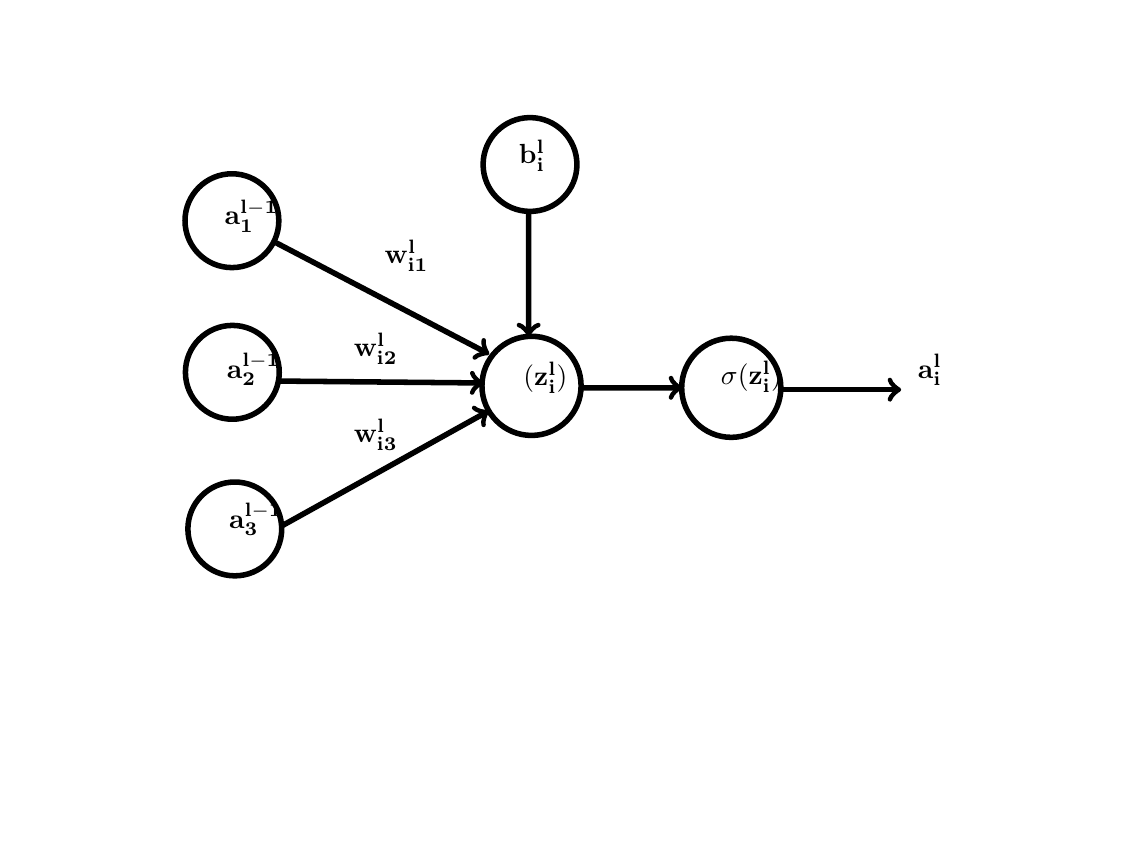
\begin{tikzpicture}[scale=0.45]
\clip(-6.836595828830608,6.483123289392461) rectangle (23.96217415591174,28.919243790057973);
\draw [line width=2pt] (-1.072323706231507,23.471677466691496) circle (1.3237949544534073cm);
\draw [line width=2pt] (-1.0606069491840735,19.192465620938574) circle (1.3237949544534078cm);
\draw [line width=2pt] (-0.9910206714855865,14.772252748878007) circle (1.3237949544534071cm);
\draw [line width=2pt] (7.383191907344222,18.810303474592057) circle (1.399052811248412cm);
\draw [->,line width=2pt] (0.1743228265392744,22.848354200306108) -- (6.19074739773739,19.704636856797183);
\draw [->,line width=2pt] (0.2014238381212479,18.945808532501925) -- (6.028141328245549,18.89160650933798);
\draw [->,line width=2pt] (0.3301962961892744,14.854828809357688) -- (6.176028930123589,18.10312152128025);
\draw (-1.4268961198642192,15.78768367201323) node[anchor=north west] {$\mathbf{a^{l-1}_{3}}$};
\draw (-1.489328259886619,20.012258480195612) node[anchor=north west] {$\mathbf{a^{l-1}_{2}}$};
\draw (-1.5517603999090188,24.340886855081994) node[anchor=north west] {$\mathbf{a^{l-1}_{1}}$};
\draw [line width=2pt] (7.34070664122771,25.05723383677692) circle (1.323794954453405cm);
\draw [->,line width=2pt] (7.30242141322907,23.73399261811972) -- (7.3010366974508285,20.206942042779783);
\draw (6.751714223070167,26.026554635686786) node[anchor=north west] {$\mathbf{b^{l}_{i}}$};
\draw [line width=2pt] (13.02020231639471,18.75610145142811) circle (1.3990528112484113cm);
\draw (12.453849678449359,19.783340633446812) node[anchor=north west] {$\mathbf{\sigma(z_{i}^{l})}$};
\draw (6.876578503114968,19.76252992010601) node[anchor=north west] {$\mathbf{(z_{i}^{l})}$};
\draw [->,line width=2pt] (8.781170177104421,18.755480797346557) -- (11.638050725714063,18.75610145142811);
\draw (2.9641643950445737,23.196297621337997) node[anchor=north west] {$\mathbf{w_{i1}^{l}}$};
\draw (2.090114434730975,18.139294279523618) node[anchor=north west] {$\mathbf{w_{i3}^{l}}$};
\draw (2.090114434730975,20.57414774039721) node[anchor=north west] {$\mathbf{w_{i2}^{l}}$};
\draw [->,line width=2pt] (14.456555930239306,18.70189942826416) -- (17.817081366404018,18.70189942826416);
\draw (18.01031014044295,19.97063705351401) node[anchor=north west] {$\mathbf{a_{i}^{l}}$};
\end{tikzpicture}
\end{frame}



\begin{frame}{Output}
\begin{equation}
a^{l}_{i} = \sigma ( \sum_{i} w_{ik}^{l}a_{i}^{l-1}+b^{l}_{i})
\end{equation}
when $l$ means the number of layer and $i$ the node.
we can write $a_{i}^{l} = \sigma(z_{i}^{l})$.

\end{frame}



\begin{frame}{Regla delta generalizada}


\end{frame}




\begin{frame}{Jensen inequality}


\end{frame}

\begin{frame}

\end{frame}



\begin{frame}{Cross entropy}


\end{frame}

\end{document}